\section{Introduction}
\label{sec:introduction}

In today's world where large datasets are stored in
terabytes and petabytes, distributed cloud computing (DCC) has become a foundation of modern technology infrastructure. As organizations generate and collect vast amounts of data in real-world scenarios such as social media \cite{ali2013cloud}, e-commerce \cite{wang2013influences}, and scientific research \cite{gunarathne2010mapreduce}, the need for efficient processing has grown exponentially. 

Recently, a form of parallel computing has emerged as a simple, reliable, and distributed paradigm for processing massive amounts of data. This paradigm, known as MapReduce, was introduced by Google in 2004 \cite{dean2008mapreduce}, which is a programming model and an associated implementation designed for processing large datasets. As one of the first systems to popularize the concept of DCC, MapReduce has been widely adopted and utilized by at least 34\% scientists all over the world \cite{kim2017data}. It is also renowned for its simplicity, scalability, and ease of use. Specifically, MapReduce divides the input data into smaller chunks and processes them in parallel across multiple machines. As illustrated in Figure~\ref{fig:mapreduce-framework}, users only need to specify a map function that processes a key/value (KV) pair to generate a set of intermediate KV pairs, and a reduce function that merges all intermediate values with respect to the same intermediate key. Therefore, this model hides the complexity of DCC, allowing users to focus on the data processing logic.

\begin{figure}
    \centering
    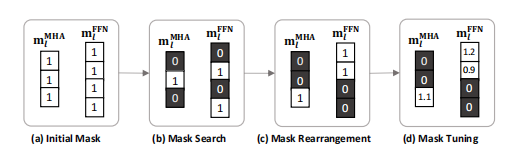
\includegraphics[width=0.5\textwidth]{framework}
    \caption{The architecture of the MapReduce framework.}
    \label{fig:mapreduce-framework}
\end{figure}

\noindent\textbf{Motivation.} Two decades after its invention, a vast amount of new DCC frameworks, such as Apache Hadoop \cite{white2012hadoop}, Apache Spark \cite{zaharia2016apache}, and Apache Flink \cite{katsifodimos2016apache}, have been proposed on top of the MapReduce model. These frameworks have further extended the capabilities of MapReduce, enabling better optimizations and performance improvements. Despite these advancements, the original MapReduce model has remained a fundamental building block for many DCC systems. Therefore, revisiting the implementation of the MapReduce framework is still of great significance. Although MapReduce offers simple and developer-friendly interfaces for deploying, i.e., map and reduce functions, its internal implementation remains complex and challenging. Delving into the internals of MapReduce can provide valuable insights into the design and optimization of modern DCC systems.

\begin{figure*}
    \centering
    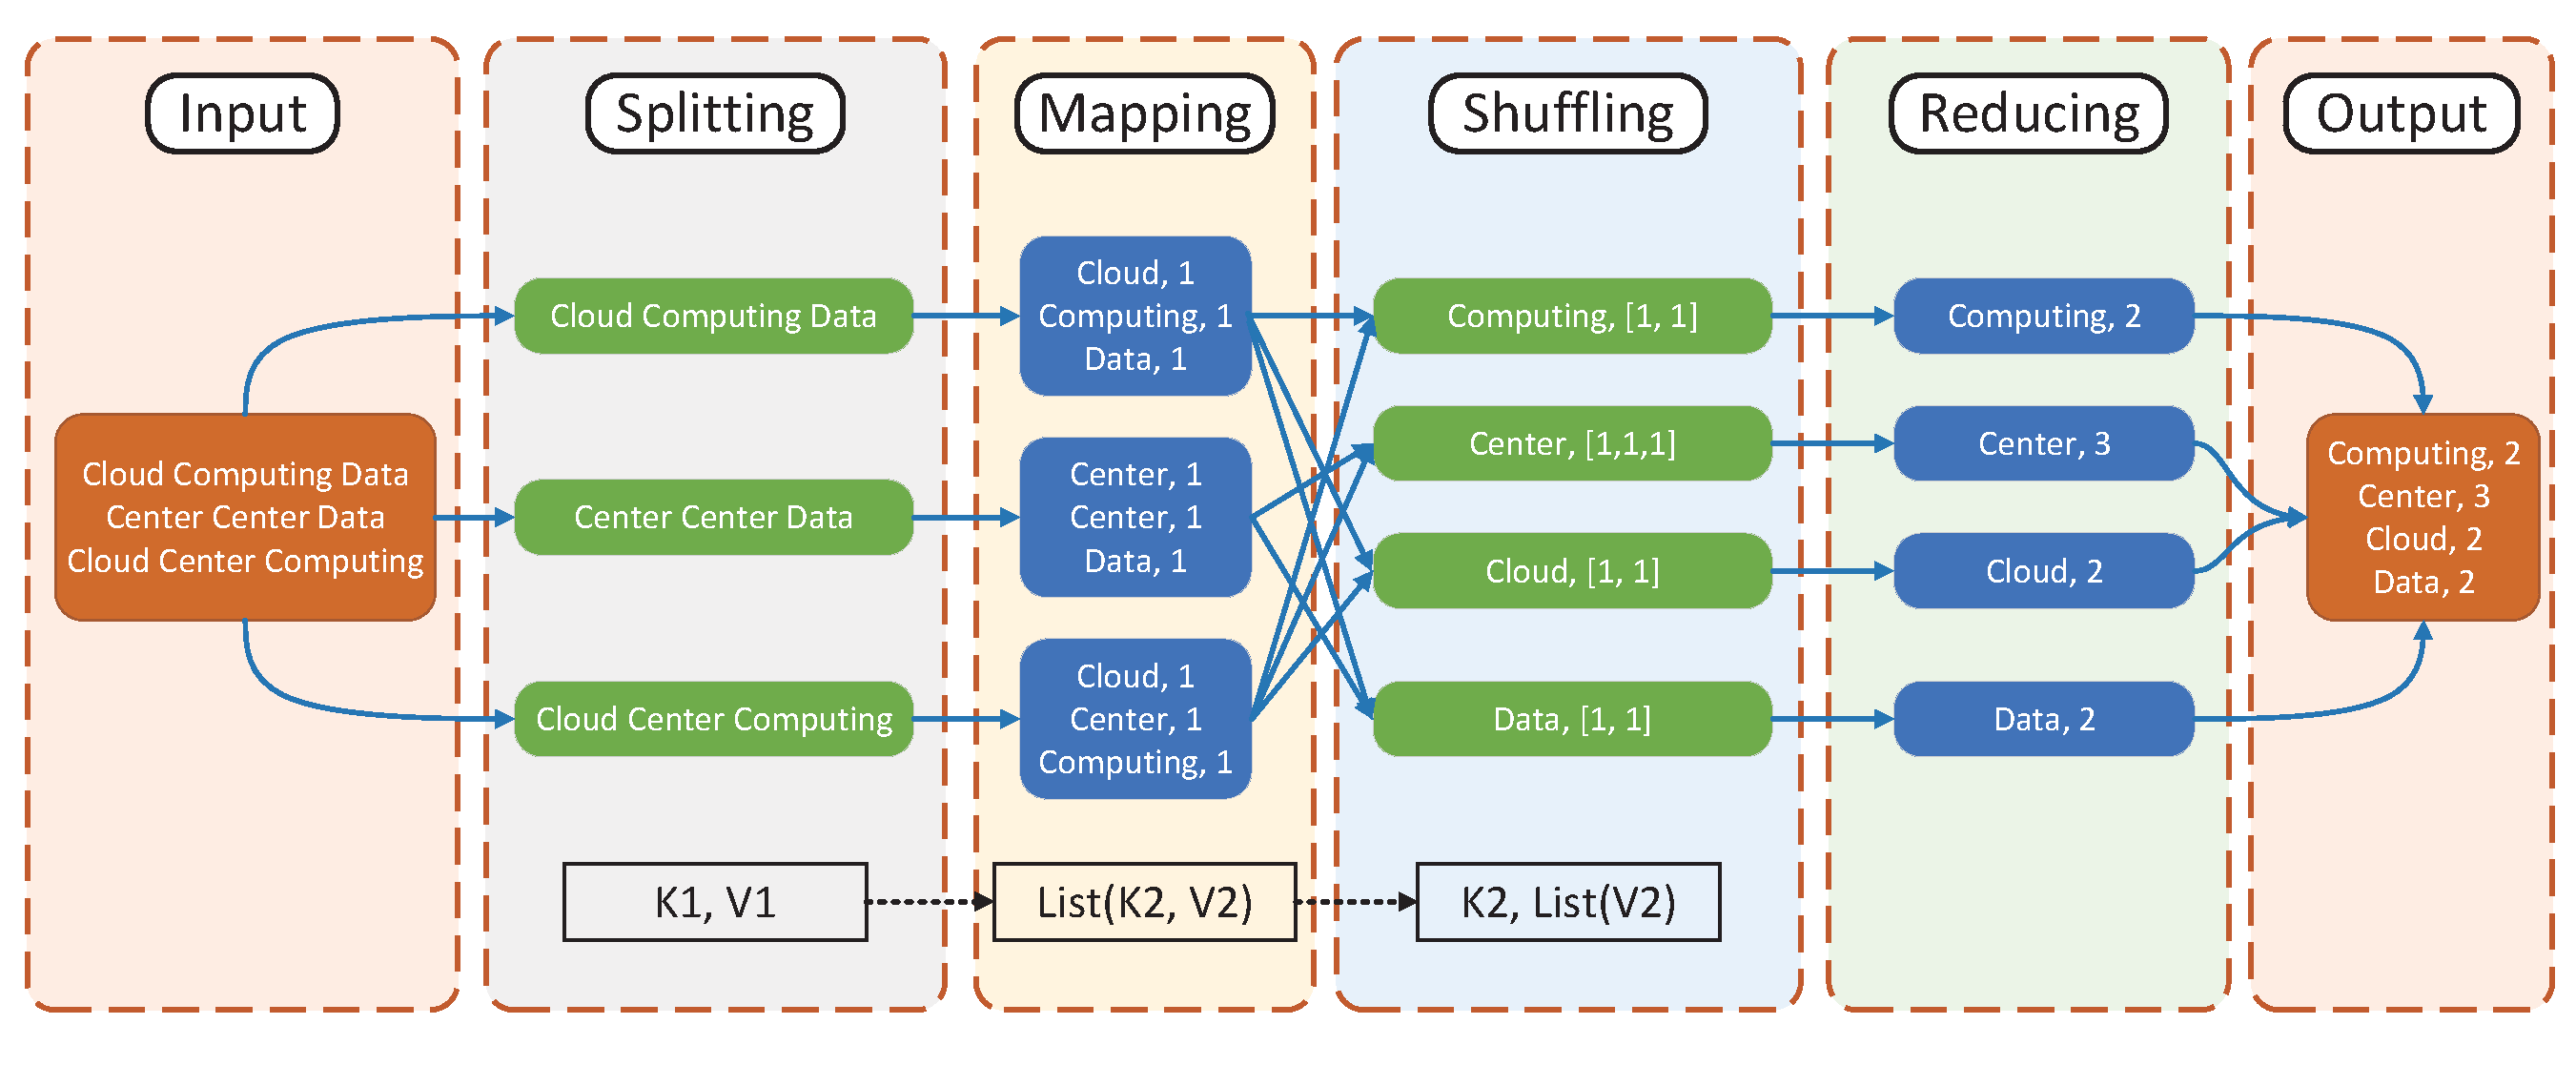
\includegraphics[width=1\textwidth]{example}
    \caption{A toy example of the MapReduce model in WordCount application.}
    \label{fig:example}
\end{figure*}

\noindent\textbf{Contributions.} In this paper, we implement a simplified, but efficient and comprehensive version of the MapReduce framework, demonstrating its correctness and efficiency through extensive experiments. Our implementation not only follows the core idea proposed in the original MapReduce paper \cite{dean2008mapreduce}, but also highlights the adaptability of the MapReduce model using several typical test cases. To sum up, the main contributions of this paper are as follows:

\begin{itemize}
    \item We give a detailed overview of the MapReduce framework in Section~\ref{sec:background}, highlighting its key components and functionalities.
    \item We present our implementation of the MapReduce framework in Section~\ref{sec:implementation}. Despite its simplicity, our implementation is efficient and capable of solving real-world problems.
    \item Furthermore, we evaluate the performance of our framework using various test cases in Section~\ref{sec:evaluation}. The results demonstrate the correctness and efficiency of our implementation.
\end{itemize}

The rest of the paper is organized as follows. Section~\ref{sec:relatedwork} discusses related work, and Section~\ref{sec:conclusion} concludes the paper.
